\documentclass{koala-fr}

\begin{document}

\title{R-Type Online}
\subtitle{USER DOCUMENTATION}
\member{Sofia Bideaux}{bideau_s@epitech.eu}
\member{Vincent Munoz}{munoz_v@epitech.eu}
\member{Idriss Moutawakil}{moutaw_i@epitech.eu}
\member{Noélie Sylvain}{sylvai_n@epitech.eu}
\member{Barbara Lepage}{lepage_b@epitech.eu}

\summary
{
  The famous scrolling shoot-em-up arcade game R-Type in a new version
  Online and Multi-player!
  \begin{figure}[H]
    \begin{center}
      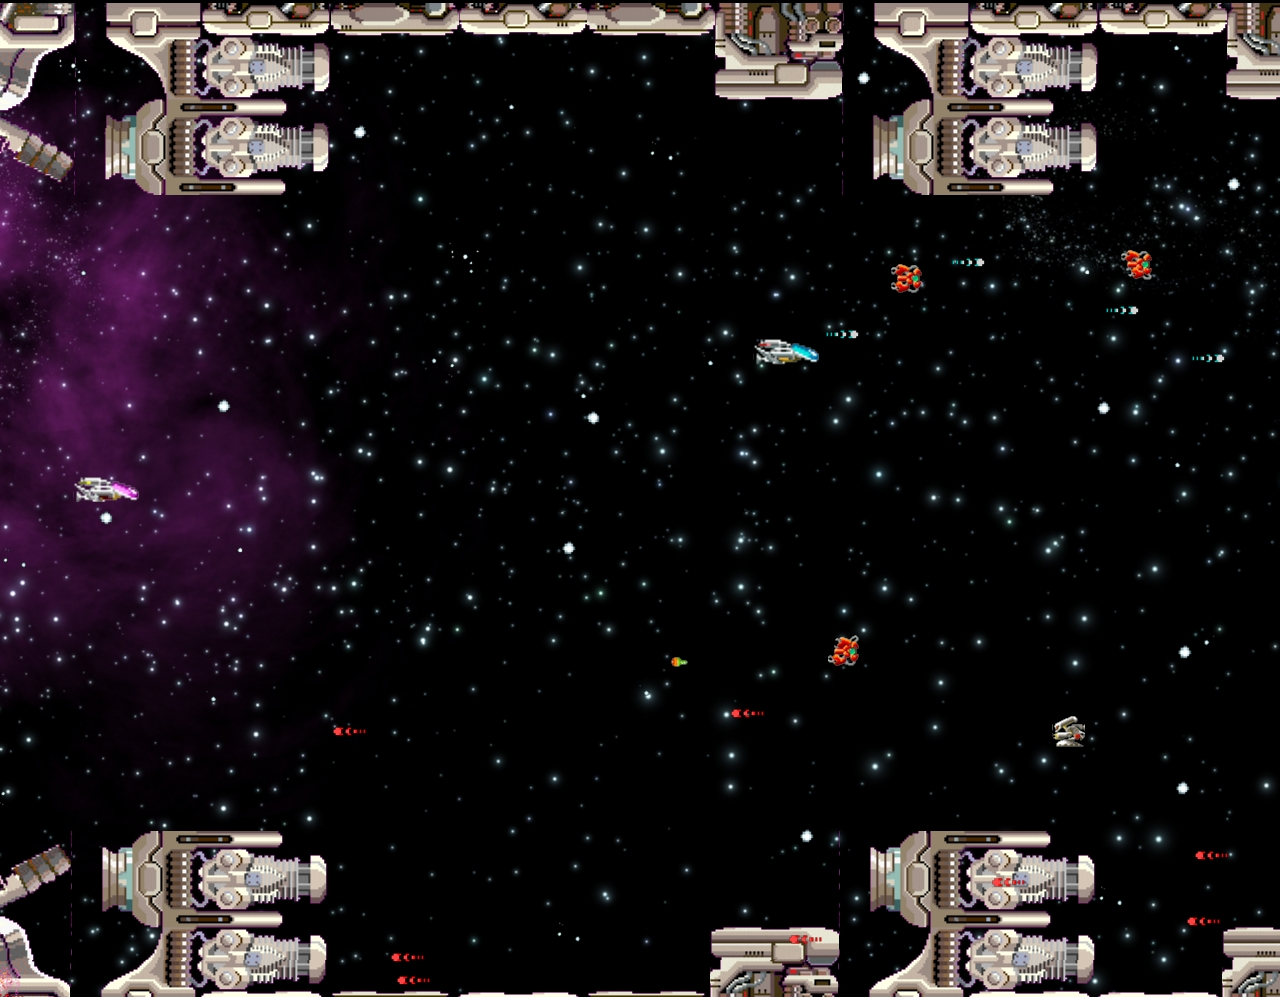
\includegraphics[width=15cm]{game.jpg}
    \end{center}
  \end{figure}
}

\maketitle

\tableofcontents

\chapter{Introduction}

\section{What is R-Type?}

R-Type is a side scrolling shoot-em-up arcade game produced by Irem in 1987. The player controls a space fighter named R-9a ``Arrowhead'' to defend humanity against a mysterious but powerful alien life-form known as ``Bydo'', which was later discovered to be not entirely alien in origin. R-Type is recognized as one of the classics of the shooter genre from the 1980s arcade.

\section{R-Type Story}

R-Type is set in the 22nd century, and the player flies a futuristic fighter craft called the R-9a ``Arrowhead'', named for its shape, and because it is the ninth model in the 'R' series of fighter craft (but it is the first of the series to actually be used in combat; the previous models were all prototypes). The mission is to 'blast off and strike the evil Bydo Empire'. The significance of the R- in the series title refers to the production code as well as the term of endearment for the player fighter craft, the ``Round Canopy''.

\section{R-Type Online Updates}

This new version provide a new dimension to the classic R-Type Game : Online Gaming in multi-player. You can launch a server and share it with friends all around the world. You can have a game up to 4 players at the same time. Non-player can watch the game. There is also a World Ranking!

\chapter{Installation}

\section{Linux}

\begin{itemize}
  \item You must compile it first.
  \item Install CMake and other dependencies libraries.
  \item Open a terminal.
  \item Move to the directory containing the sources using \texttt{cd}.
  \item Type :
    \begin{lstlisting}
      #> cmake .
      #> make
    \end{lstlisting}
  \item If compilation fails, it means :
    \begin{itemize}
      \item Some libraries are missing.
      \item Your operating system is not compatible.
    \end{itemize}
\end{itemize}

\section{Windows}

%%todo

\begin{itemize}
  \item Download Installer and CMake.
  \item Launch Installer.
  \item It ask you ``Where is the source code?''. Select the directory where the R-Type source code is.
  \item It ask you ``Where to buold the binary?''. Select the directory where you want the binary (``.exe'' file) to be.
  \item Click on ``Configure''.
  \item Choose the ``Virtual Studio'' compiler.
  \item When it is finished, click on ``Generate''.
\end{itemize}


\chapter{Start Server}

\section{Linux}

\begin{itemize}
  \item Open a terminal.
  \item Move to the directory containing the sources using \texttt{cd}.
  \item Type :
    \begin{lstlisting}
      #> ./bin/server
    \end{lstlisting}
  \item If you want to launch it in the background, type :
    \begin{lstlisting}
      #> ./bin/server &
    \end{lstlisting}
    Or, if you want it to stay launched even if you close the current terminal :
    \begin{lstlisting}
      #> screen ./bin/server
    \end{lstlisting}
\end{itemize}

\section{Windows}

Double-click on the server.exe file generated by the compiler.

\chapter{Start Game}

\section{Linux}

\begin{itemize}
  \item Open a terminal.
  \item Move to the directory containing the sources using \texttt{cd}.
  \item Type :
    \begin{lstlisting}
      #> ./bin/client
    \end{lstlisting}
\end{itemize}

\section{Windows}

Double-click on the client.exe file generated by the compiler.

\section{Problem?}

If it is not working, it means :
\begin{itemize}
  \item You have not correctly set your graphic card configuration.
  \item The executable is not compiled for your architecture, you must compile it again (see "Installation" part).
  \item The game is not compatible for your operating system.
\end{itemize}

\chapter{Controllers}
See next page.

\newpage
\begin{figure}[H]
      \begin{center}
        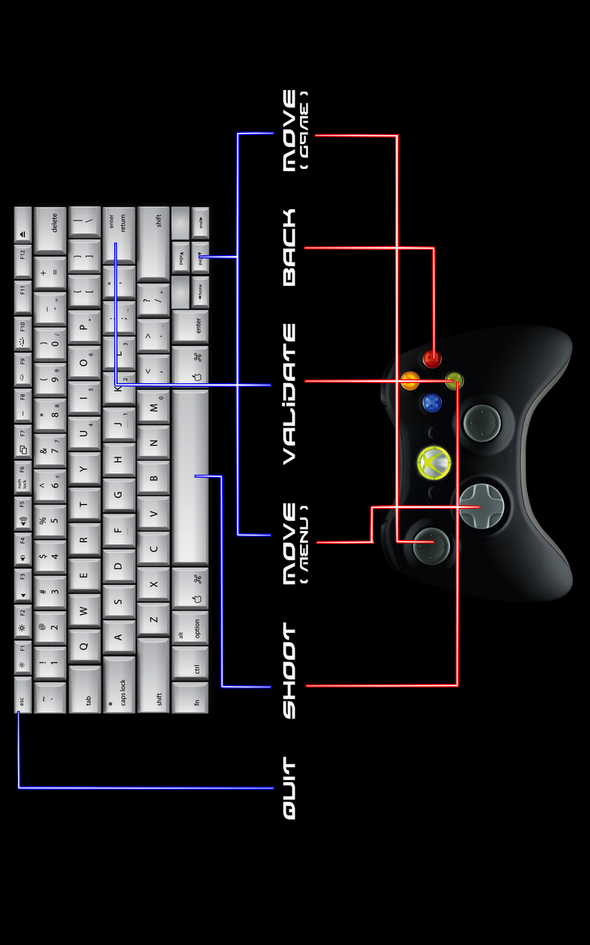
\includegraphics[width=15cm]{help.png}
      \end{center}
    \end{figure}

\chapter{Game Usage}

\section{Join Game}

\begin{itemize}
  \item Launch the game.
  \item The menu appears :
\begin{figure}[H]
      \begin{center}
        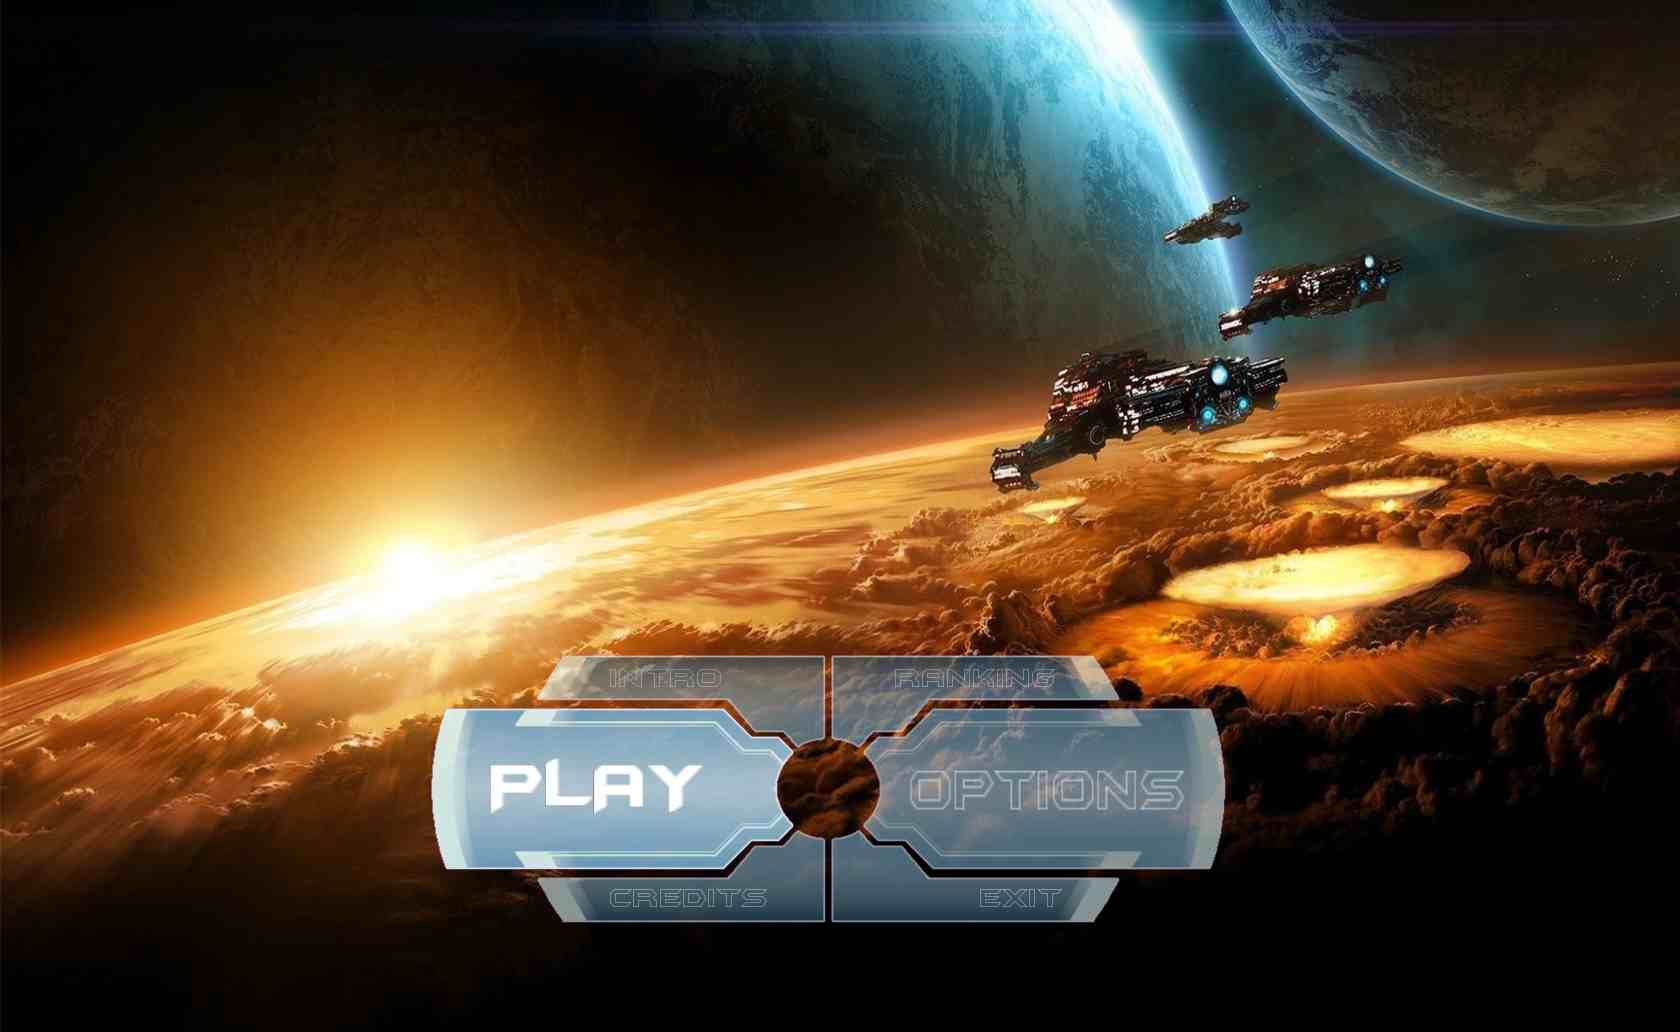
\includegraphics[width=15cm]{menu.jpg}
      \end{center}
    \end{figure}    
  \item Select the ``Play'' button.
  \item The list of games appears :
\begin{figure}[H]
      \begin{center}
        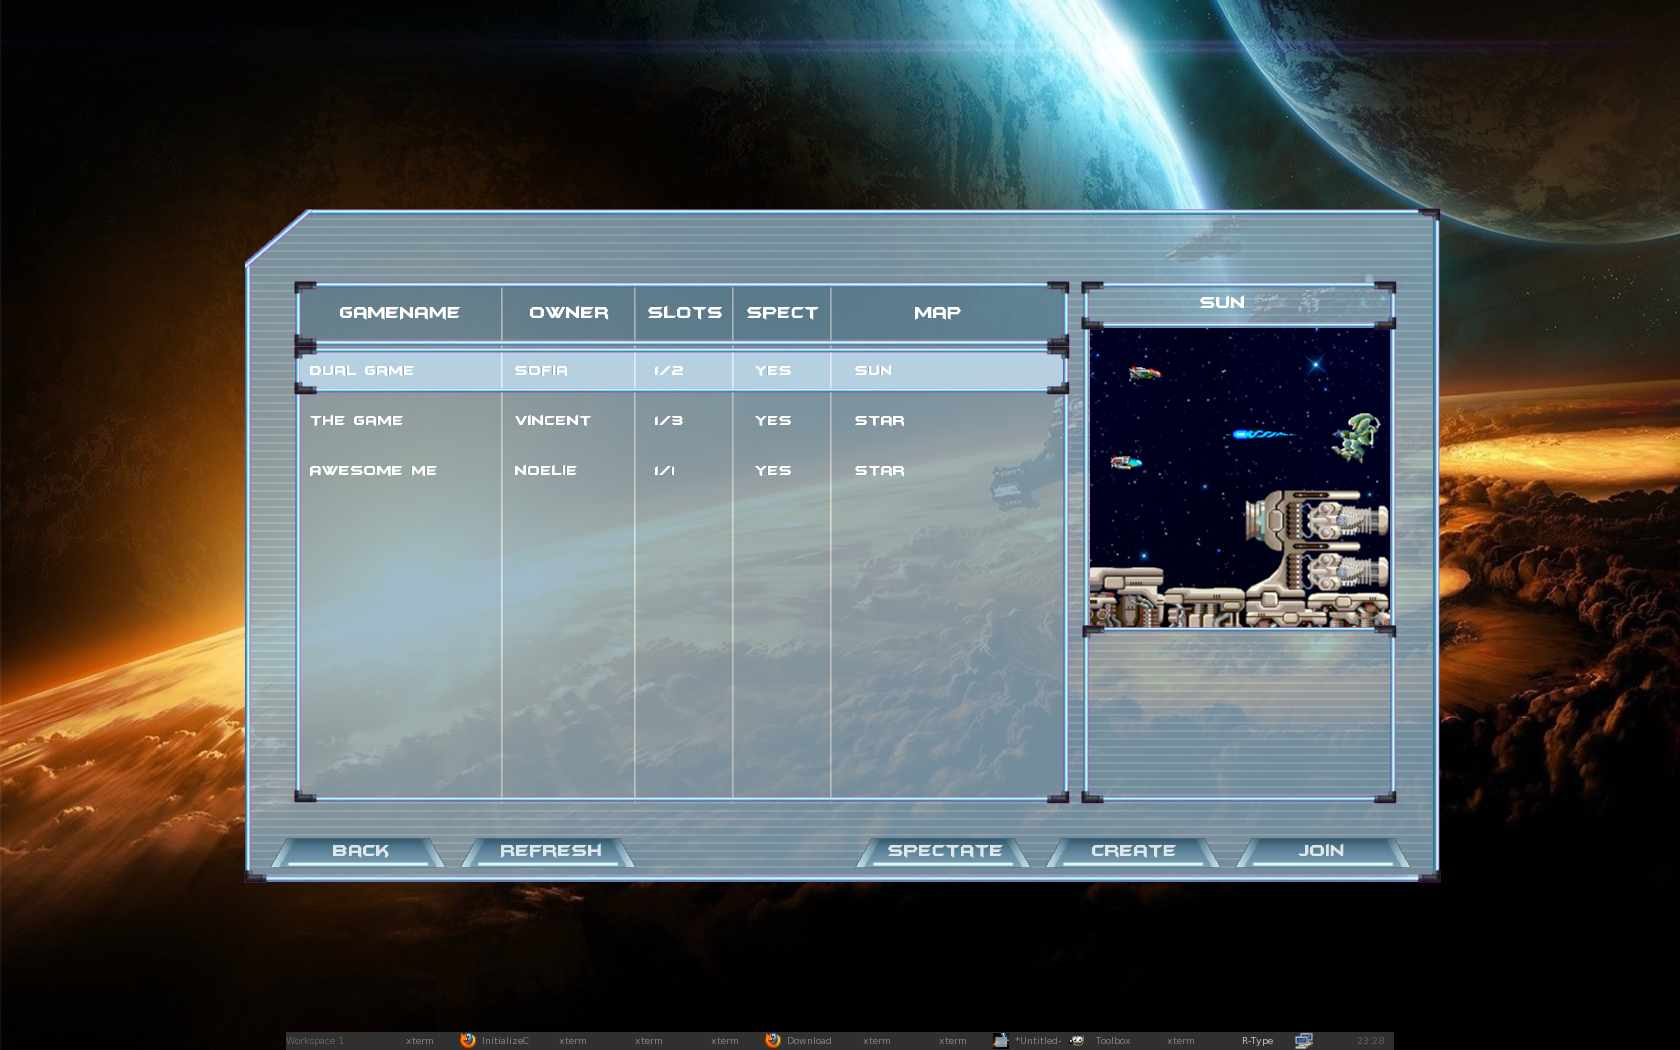
\includegraphics[width=15cm]{list.jpg}
      \end{center}
    \end{figure}
  \item Select a game.
  \item The game lobby appears :
\begin{figure}[H]
      \begin{center}
        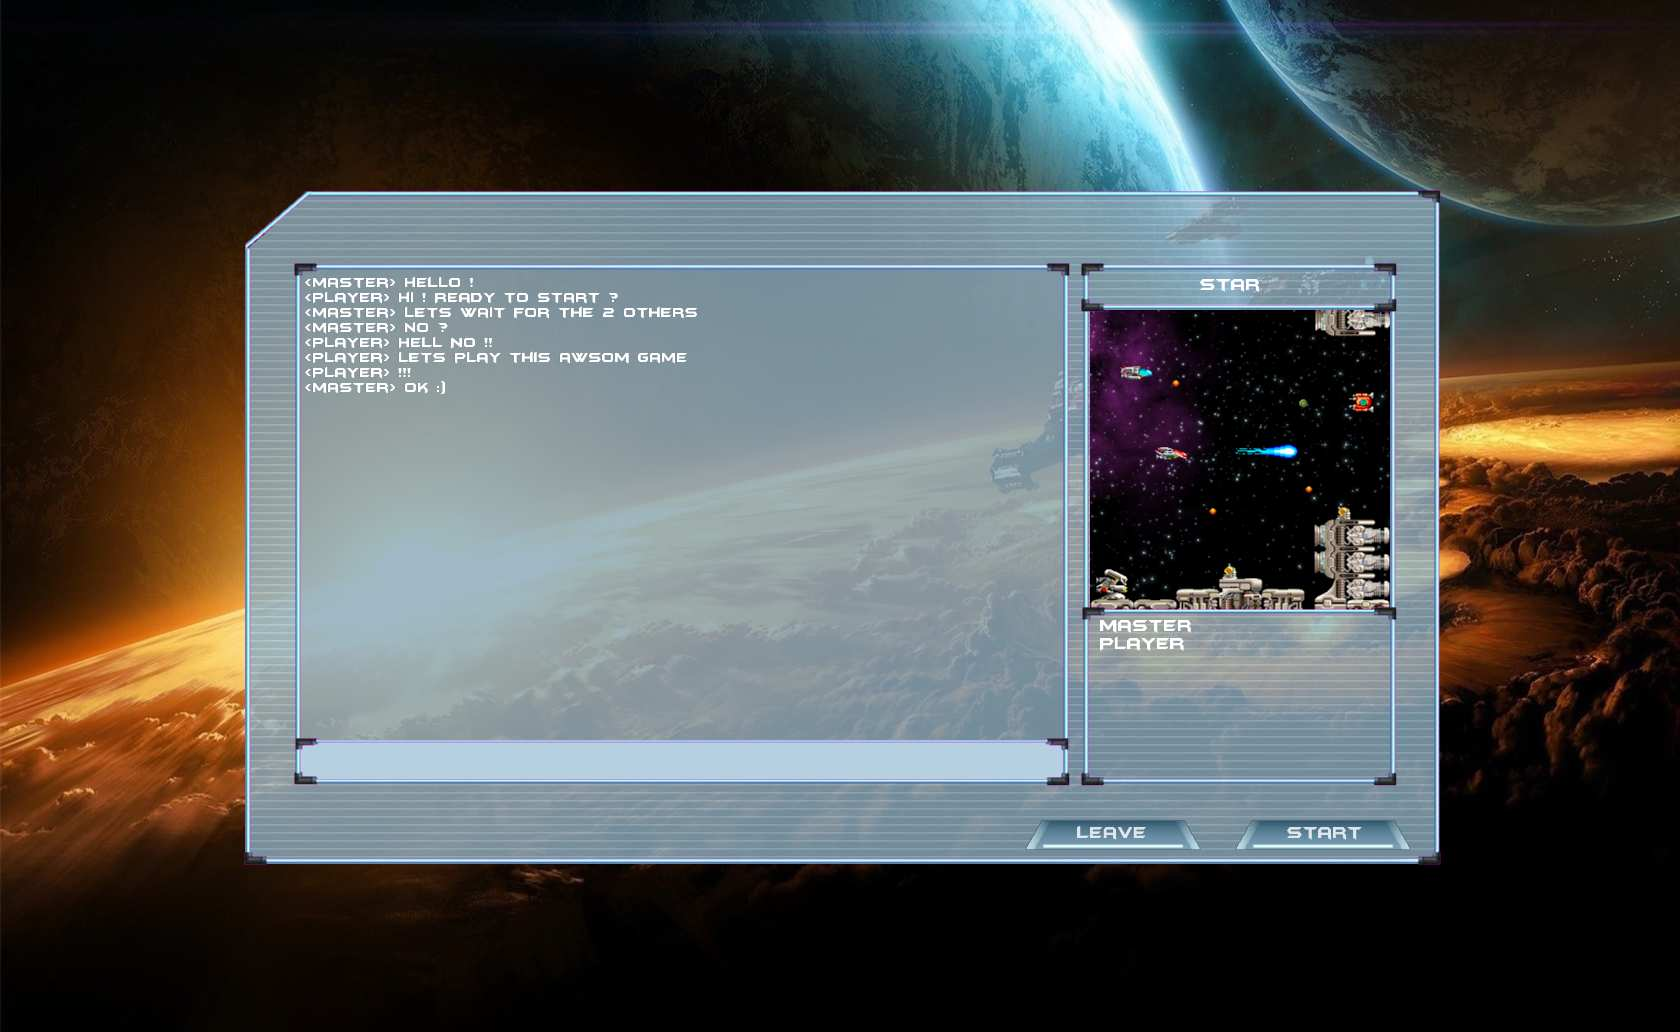
\includegraphics[width=15cm]{lobby.jpg}
      \end{center}
    \end{figure}
  \item You can now chat with other players.
  \item When the owner of the game is ready, the game will start.
\end{itemize}

\section{Create Game}

\begin{itemize}
  \item Launch the game.
  \item The menu appears :
\begin{figure}[H]
      \begin{center}
        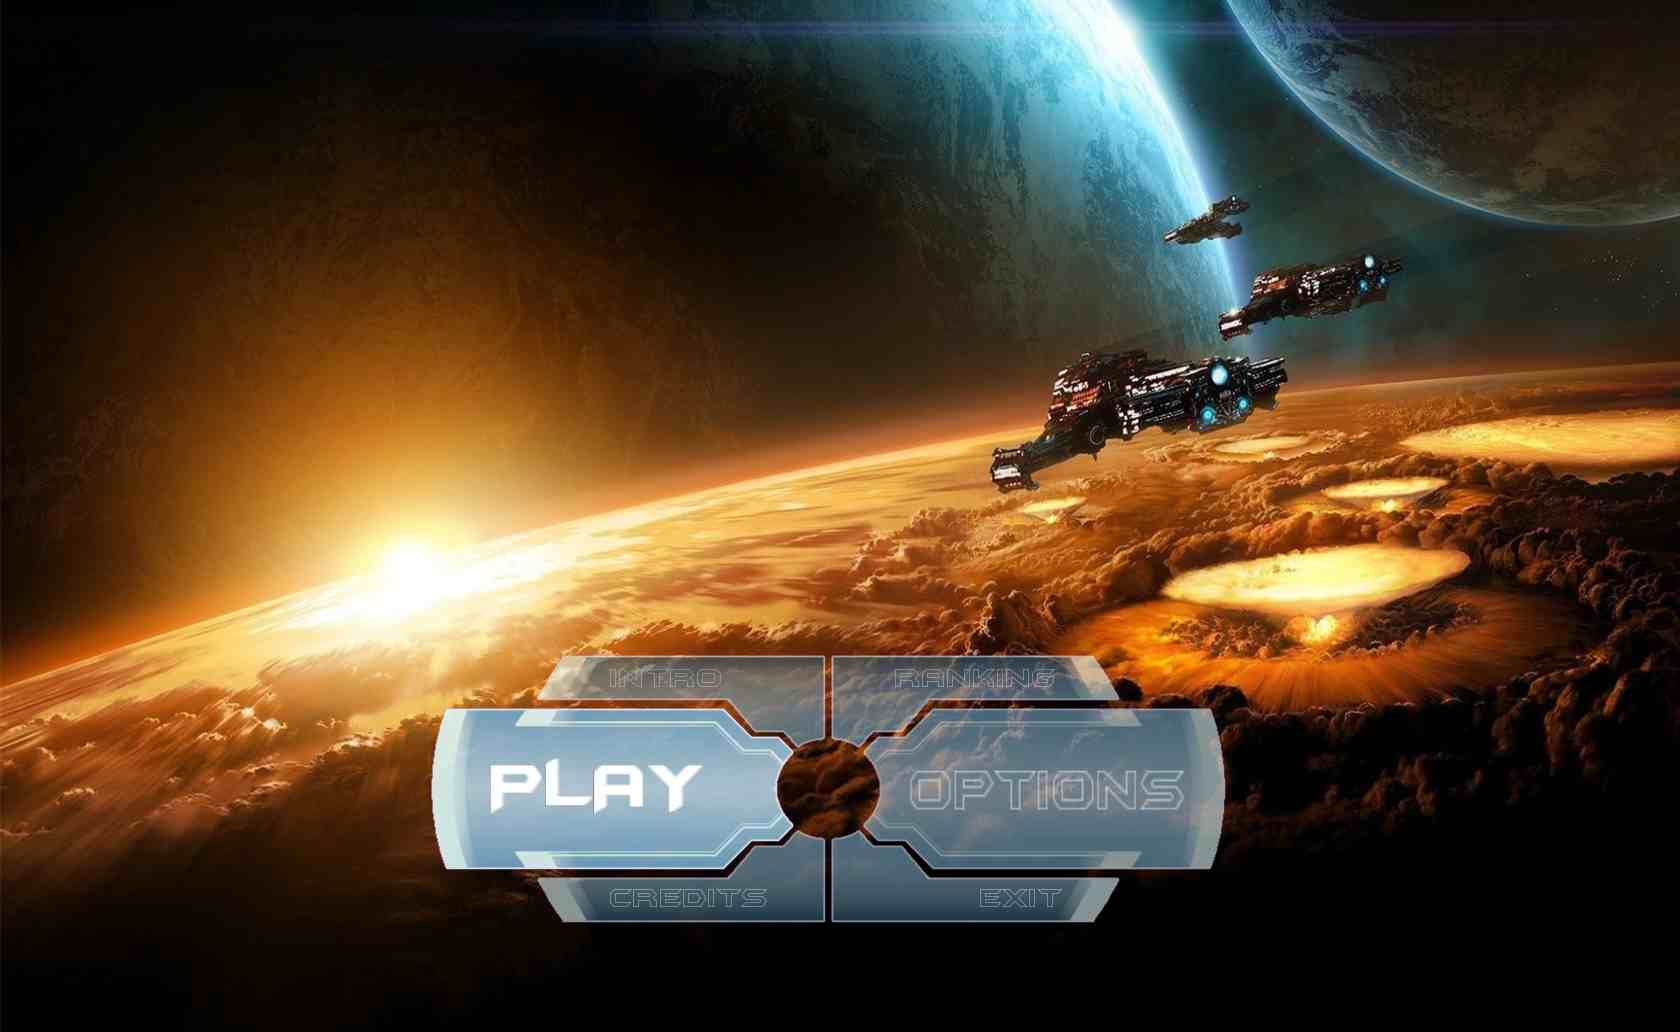
\includegraphics[width=15cm]{menu.jpg}
      \end{center}
    \end{figure}    
  \item Select the ``Play'' button.
  \item The list of games appears :
\begin{figure}[H]
      \begin{center}
        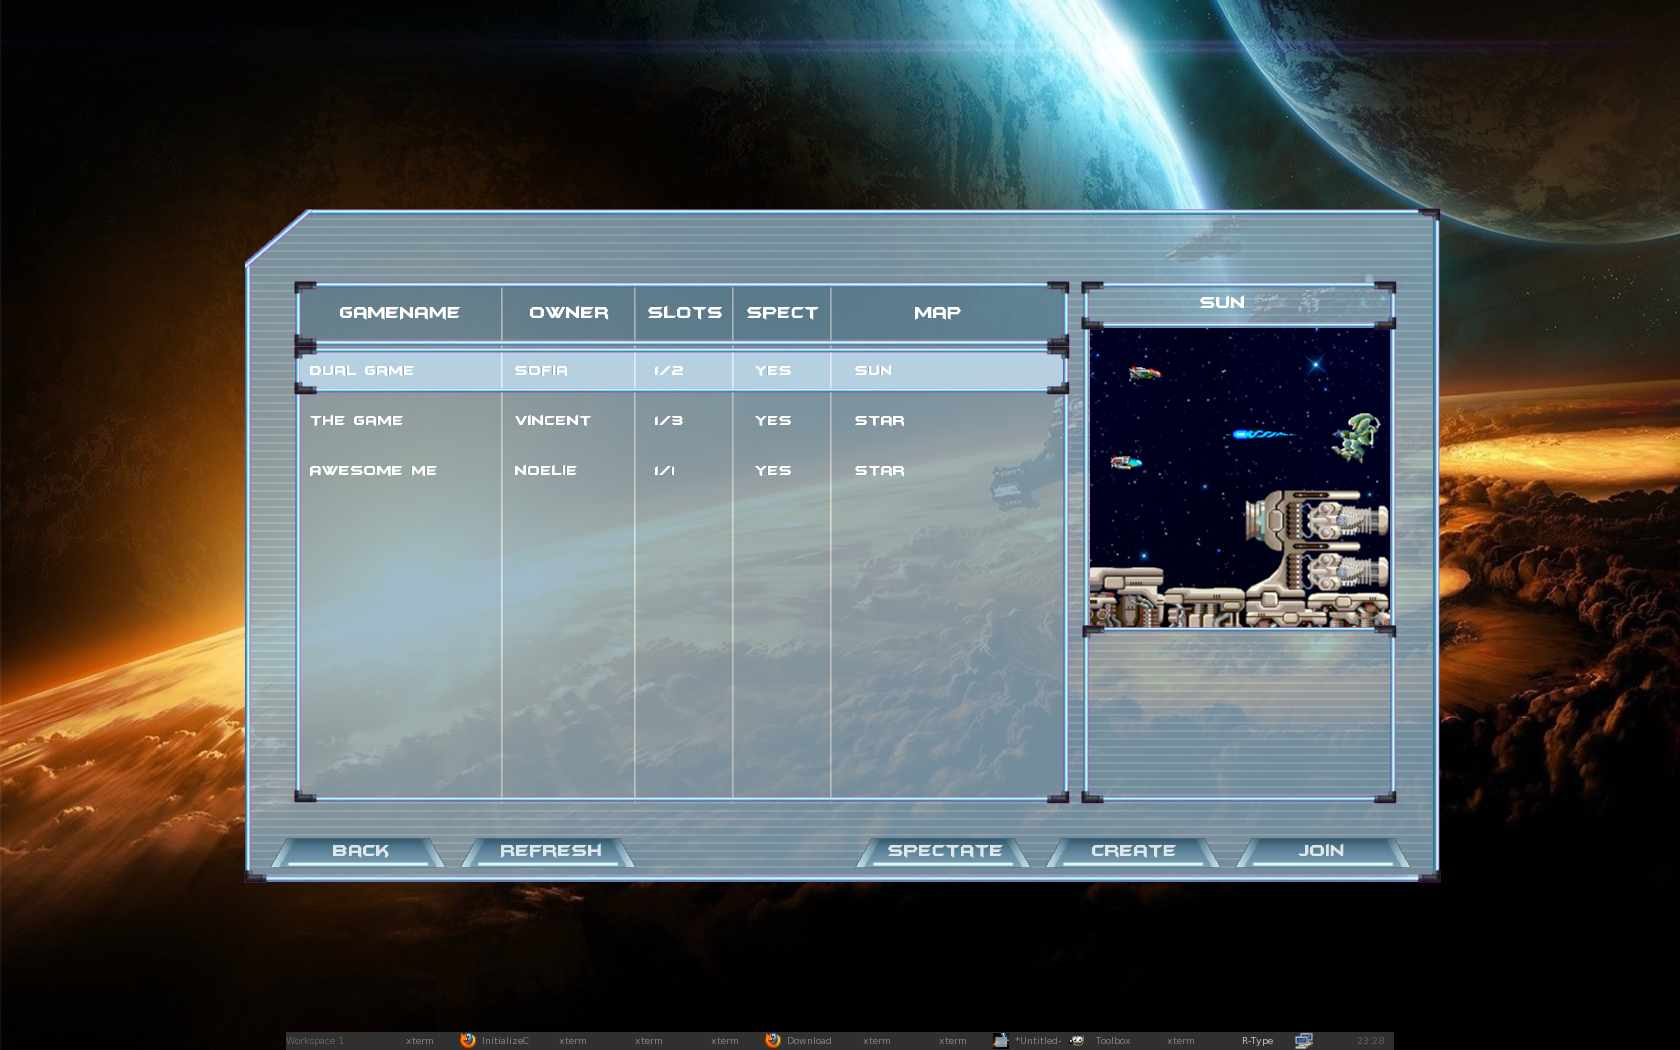
\includegraphics[width=15cm]{list.jpg}
      \end{center}
    \end{figure}
  \item Select the ``Create'' button.
  \item The Game Creation Menu appears :
\begin{figure}[H]
      \begin{center}
        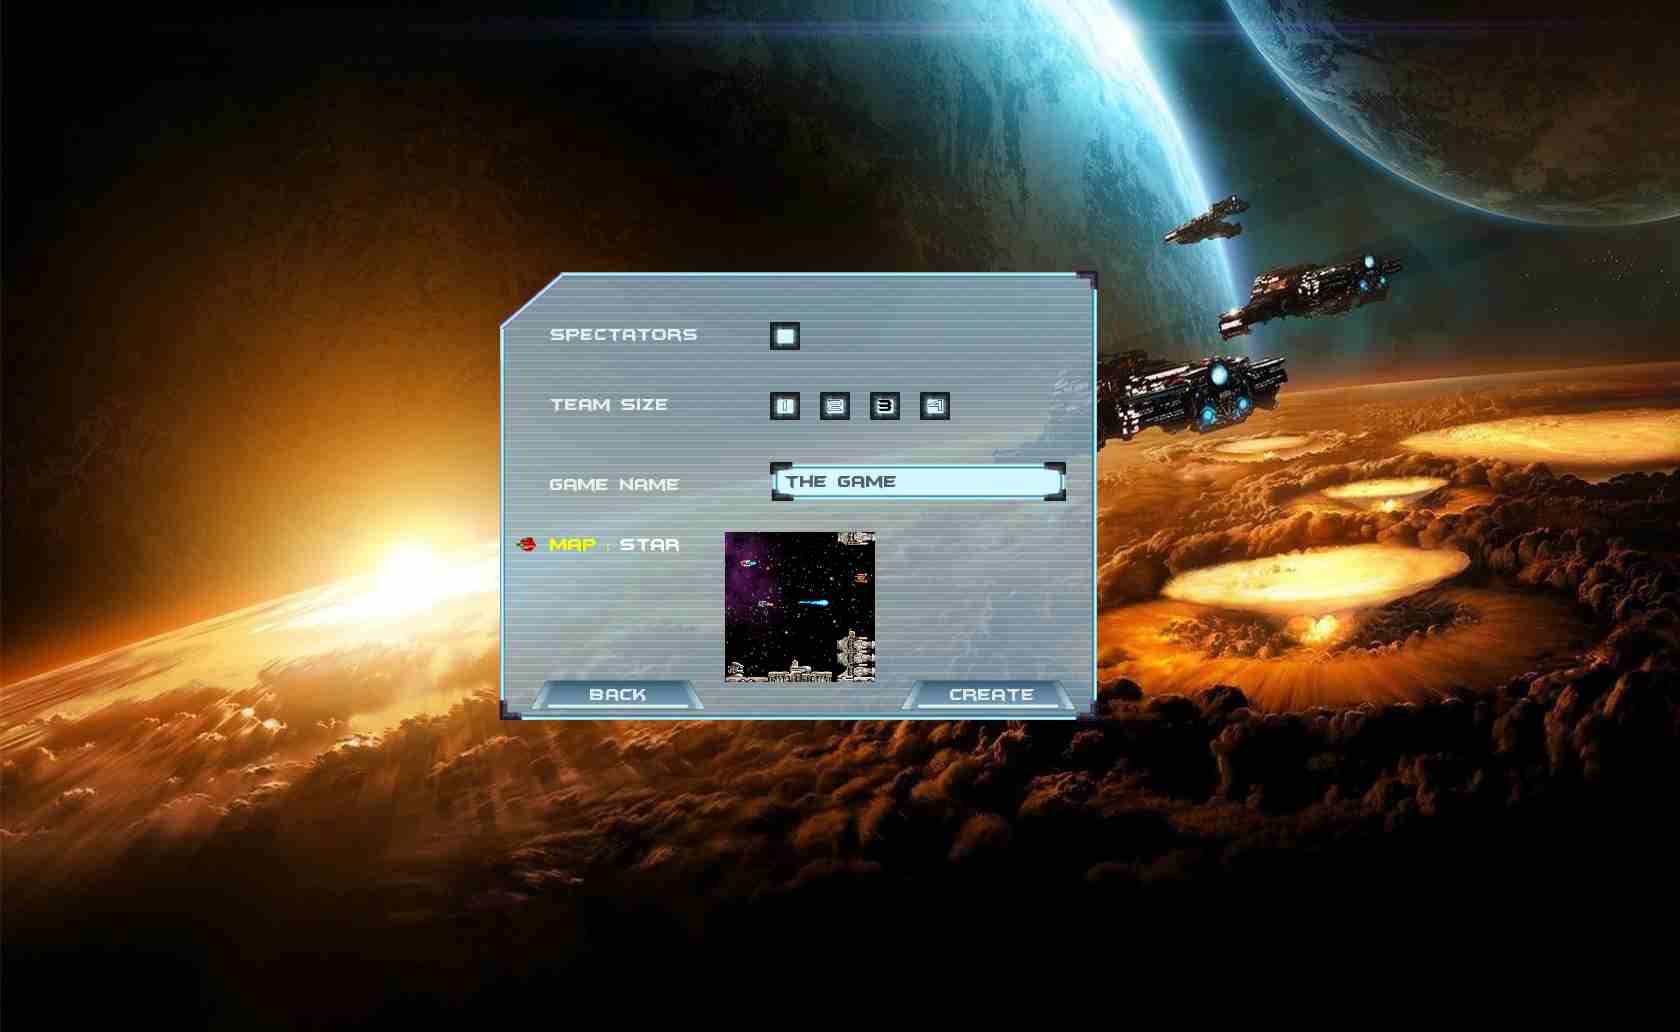
\includegraphics[width=15cm]{create.jpg}
      \end{center}
    \end{figure}
  \item Set the settings you want :
    \begin{itemize}
      \item The ``Spectators'' checkbox allow you to choose if non-player can watch the game without playing or not.
      \item The team size is the maximum player you want in this game.
      \item The game name is an identifier that you can give to your friends so they will know which game they have to join to play with you.
      \item They are several maps available. Choose your favorite!
    \end{itemize}
  \item Select the ``Create'' button.
  \item The game lobby appears :
\begin{figure}[H]
      \begin{center}
        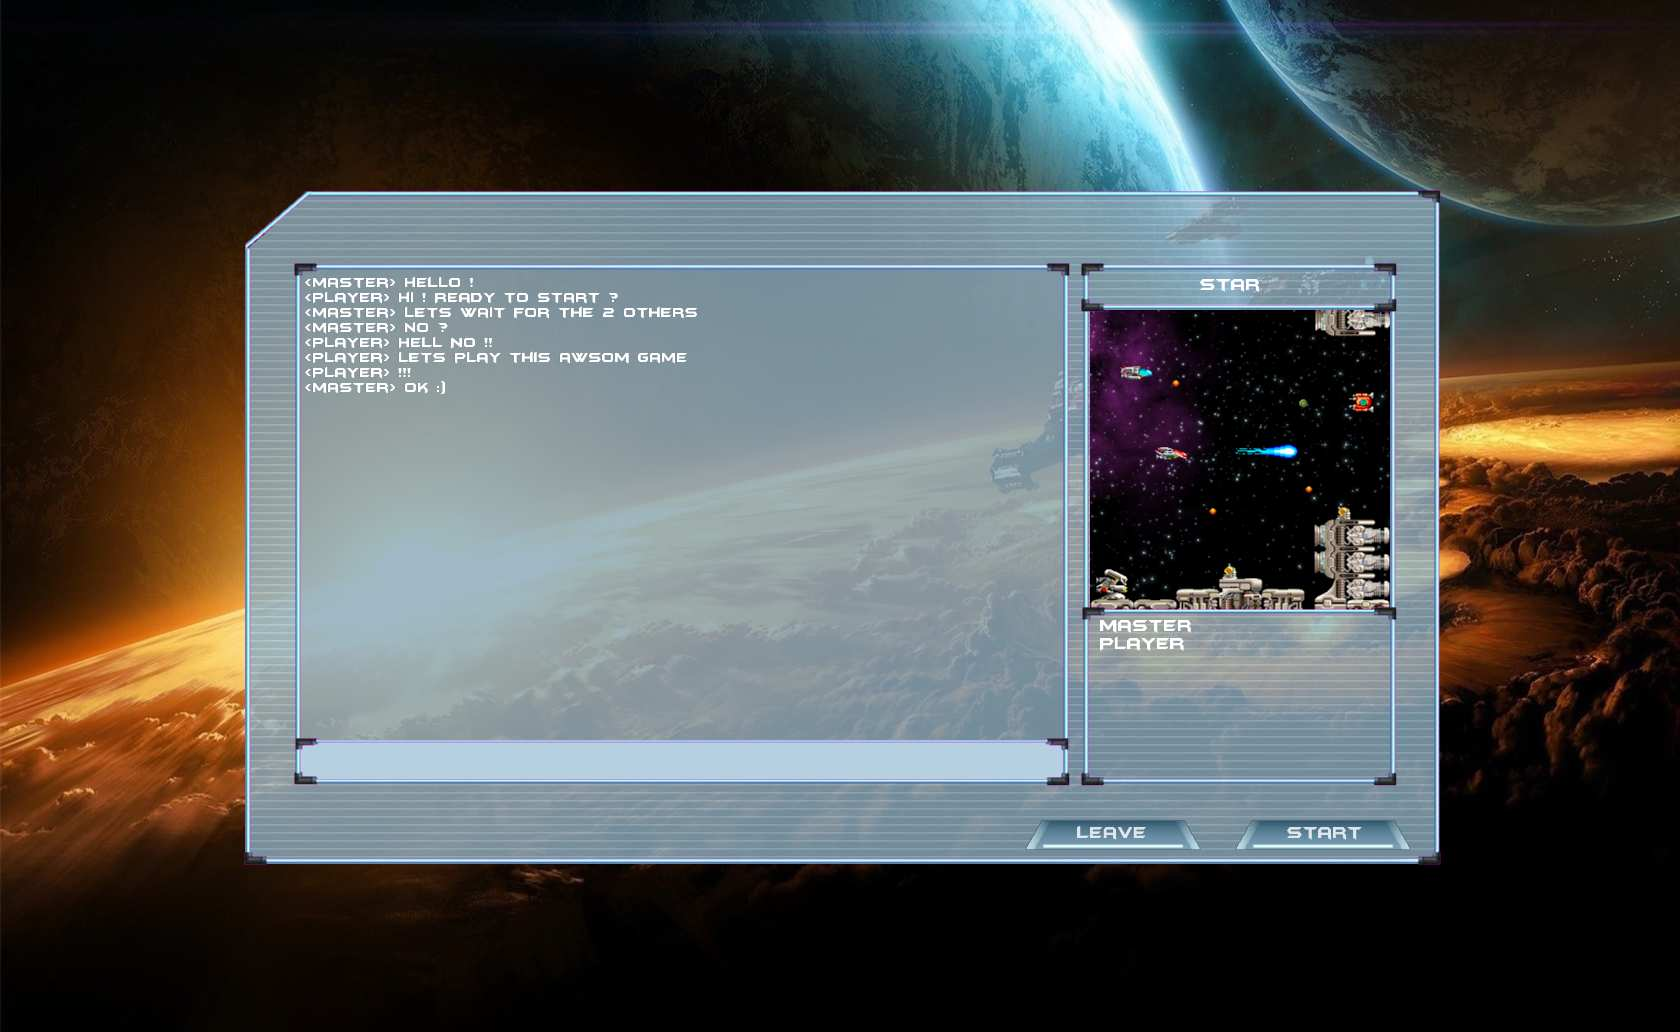
\includegraphics[width=15cm]{lobby.jpg}
      \end{center}
    \end{figure}
  \item You can now chat with other players.
  \item When you are ready, select the ``Start'' button.
  \item The game start!
\end{itemize}

\section{Play Game}

\begin{figure}[H]
      \begin{center}
        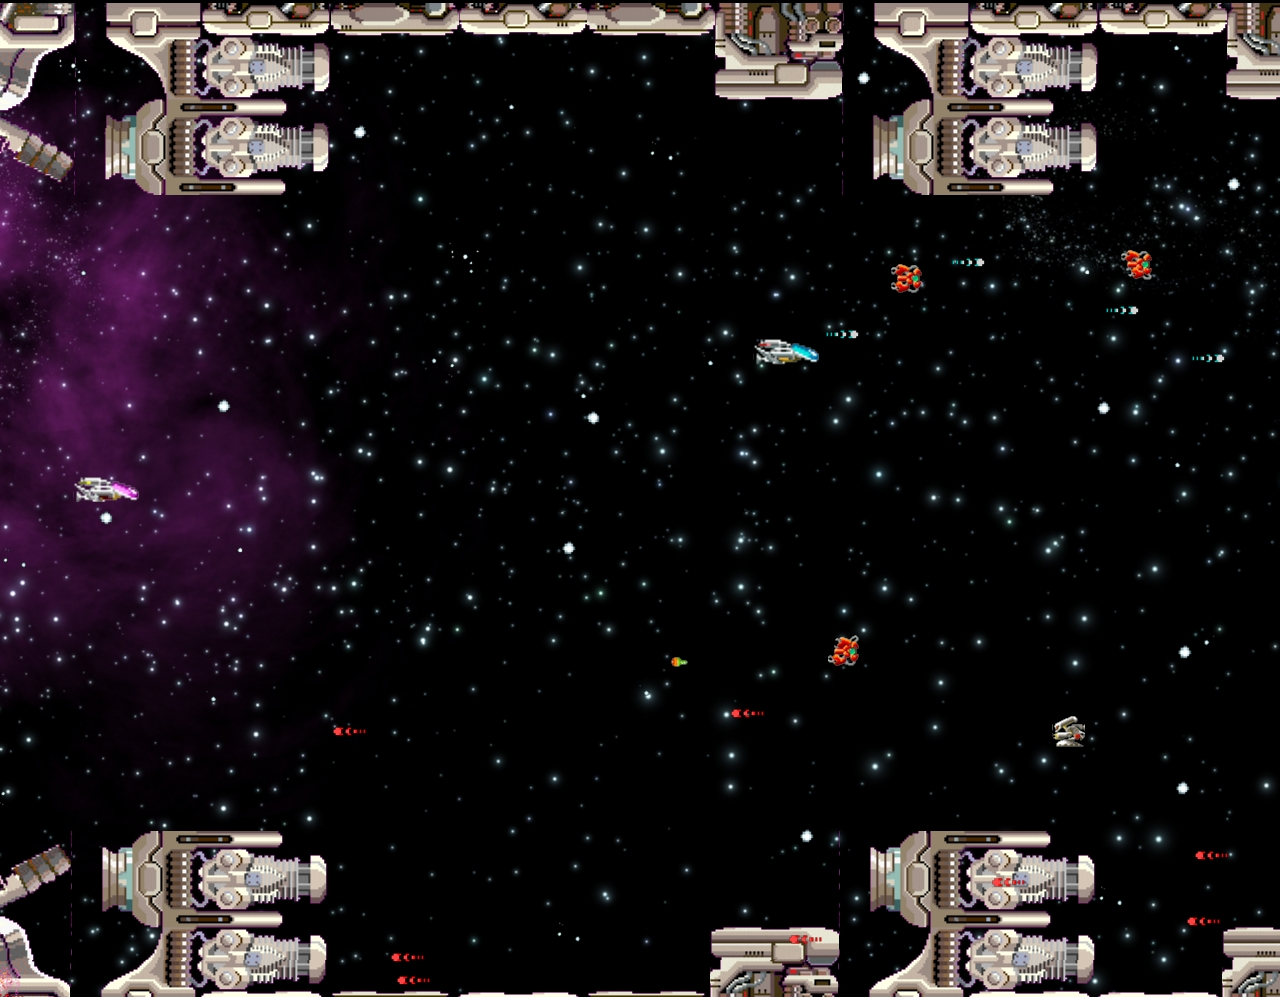
\includegraphics[width=15cm]{game.jpg}
      \end{center}
    \end{figure}
\begin{itemize}
  \item See ``Controllers'' part to know which buttons or keys you must use.
  \item Move your spaceship to avoid enemy and their bullets.
    \begin{figure}[H]
      \begin{center}
        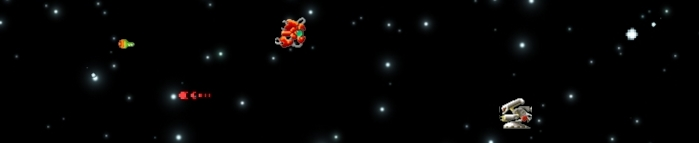
\includegraphics[width=15cm]{enemys.jpg}
      \end{center}
    \end{figure}
  \item Be carrefull of not touching ground or ceiling of the map.
    \begin{figure}[H]
      \begin{center}
        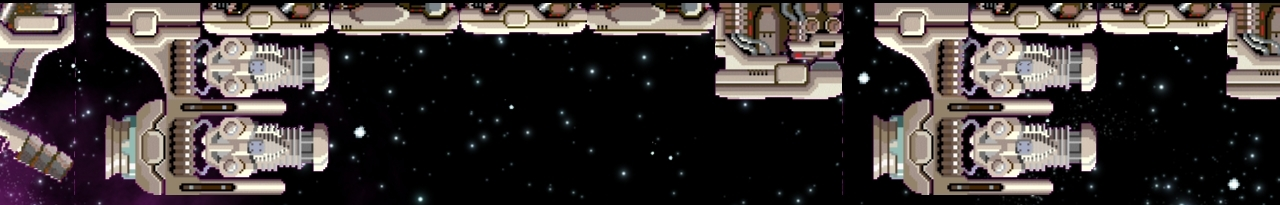
\includegraphics[width=15cm]{decor.jpg}
      \end{center}
    \end{figure}
  \item Fire enemies using the shoot button.
    \begin{figure}[H]
      \begin{center}
        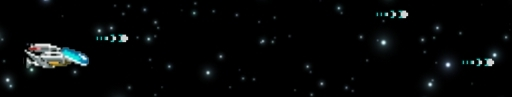
\includegraphics[width=15cm]{ownbullet.jpg}
      \end{center}
    \end{figure}
  \item When an enemy receive one of your bullet or one of the other players bullet, it died and you get points.
    \begin{figure}[H]
      \begin{center}
        
\includegraphics[width=4cm]{scores.jpg}
      \end{center}
    \end{figure}    
  \item You must play in team against the enemies.
  \item The winner is the last alive.
  \item You have some ``lifes''. Everytime an ennemy's bullet touch you, you lost one.
    \begin{figure}[H]
      \begin{center}
        
\includegraphics[width=6cm]{lifes.jpg}
      \end{center}
    \end{figure}
  \item If you lose all your lifes, you lost the game.
  \item When you lost, you can watch other players.
  \item When all players lost, the game is over :
    \begin{figure}[H]
      \begin{center}
        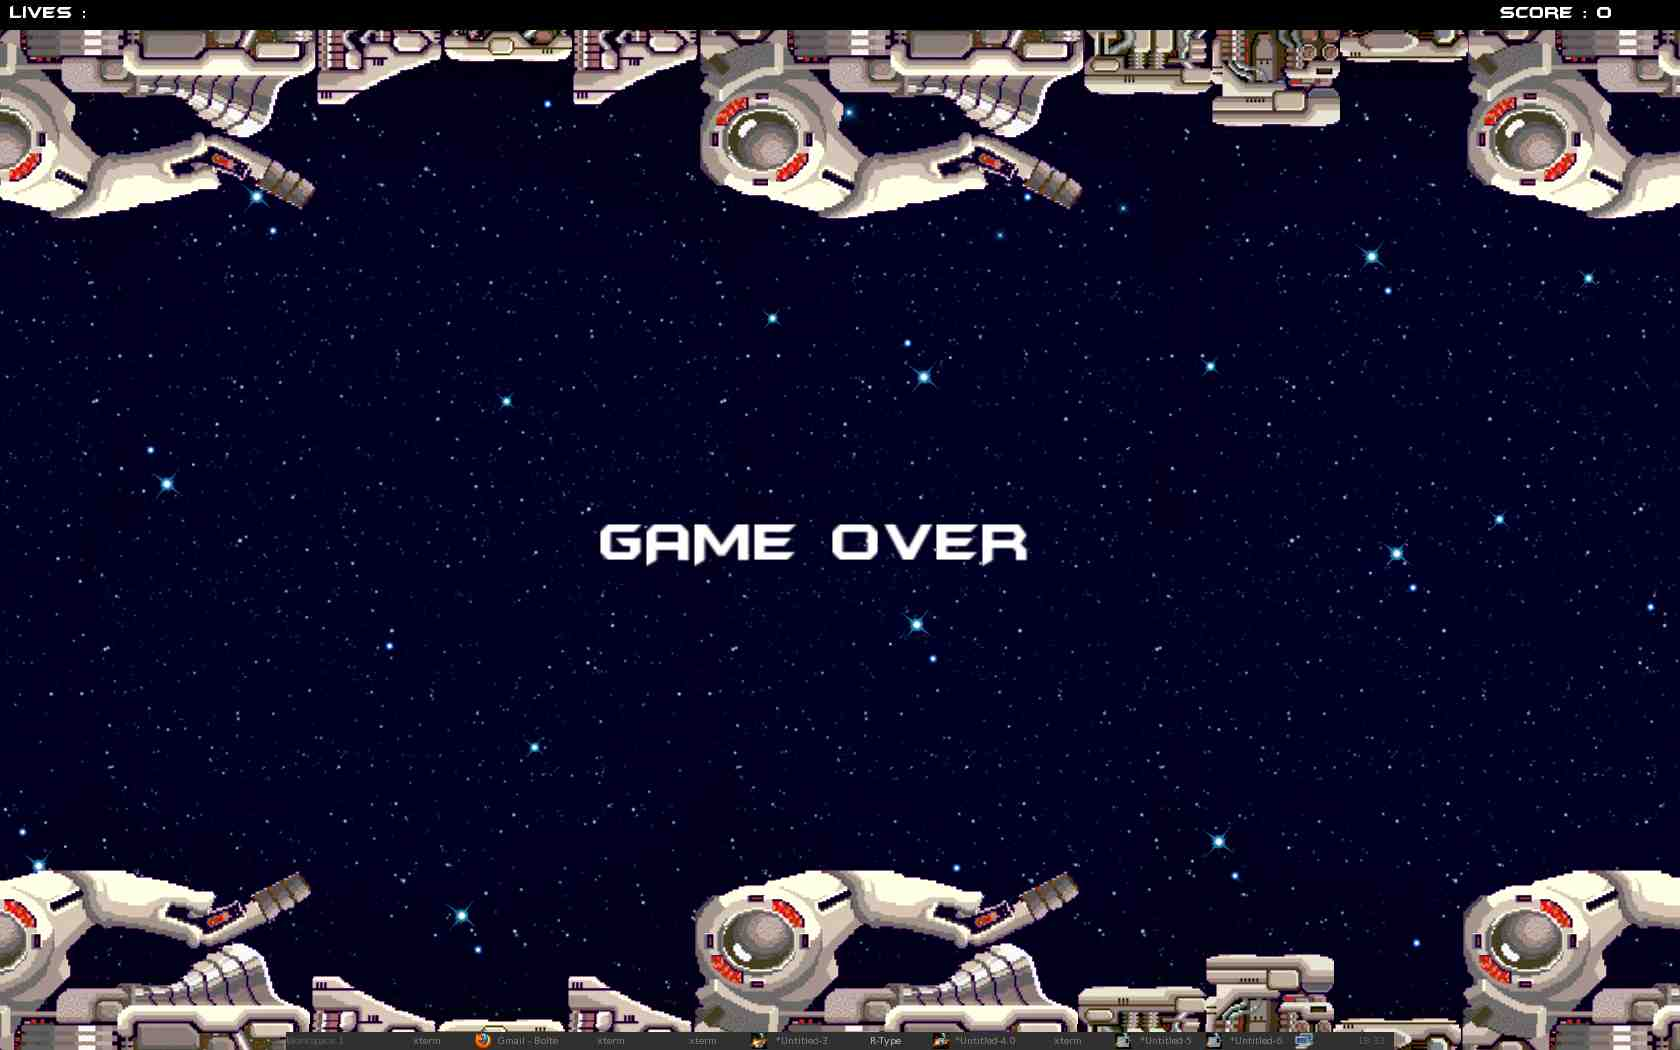
\includegraphics[width=15cm]{gameover.jpg}
      \end{center}
    \end{figure}
\end{itemize}

\chapter{Settings}

\section{Global Configuration}

\begin{itemize}
  \item Launch the game.
  \item The menu appears :
    \begin{figure}[H]
      \begin{center}
        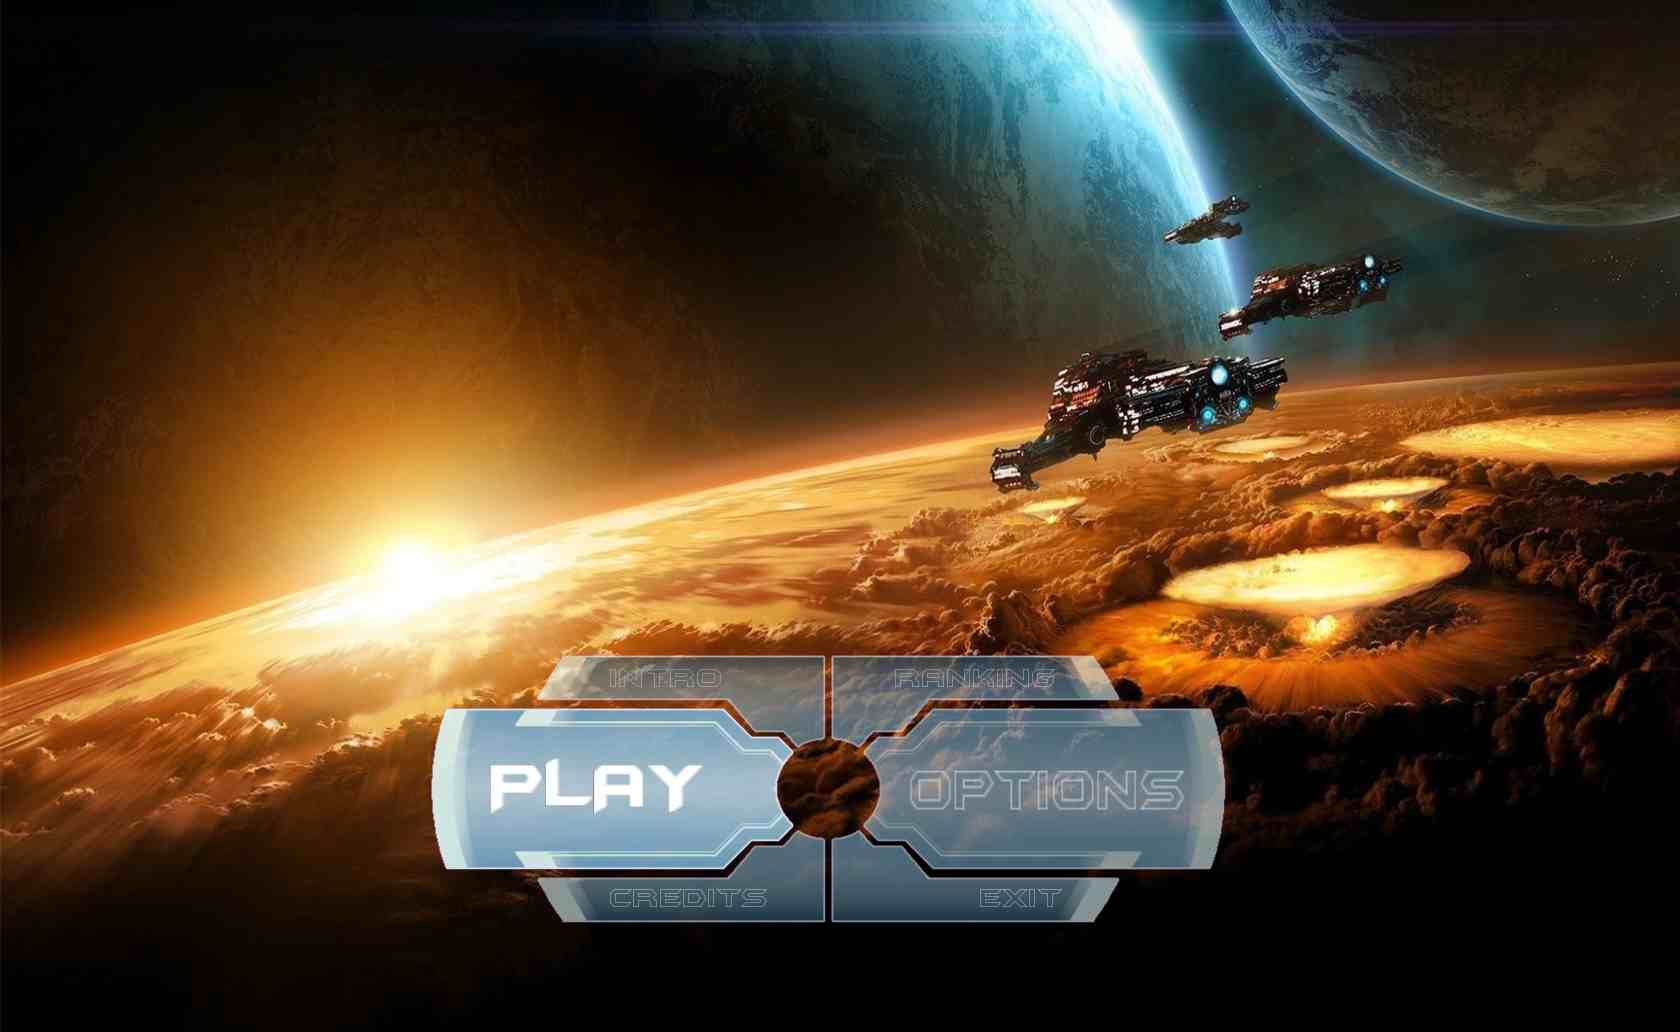
\includegraphics[width=15cm]{menu.jpg}
      \end{center}
    \end{figure}
  \item Select the ``Options'' button.
  \item The Options menu appears :
    \begin{figure}[H]
      \begin{center}
        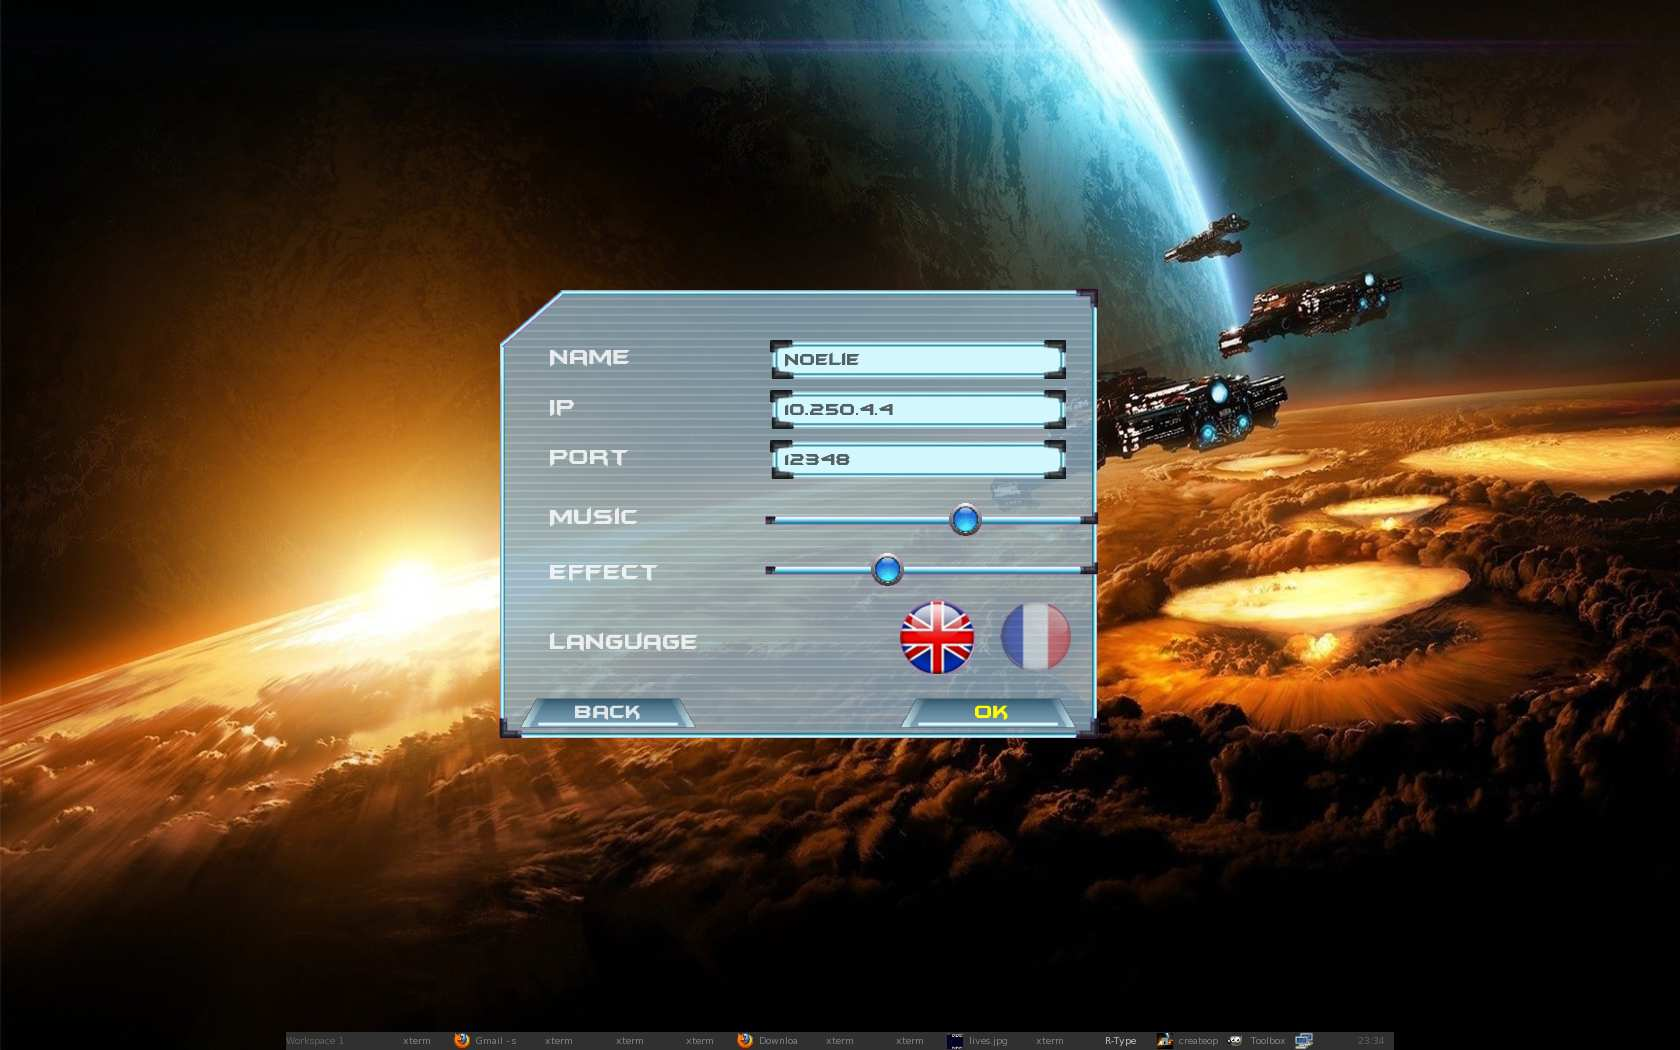
\includegraphics[width=15cm]{settings.jpg}
      \end{center}
    \end{figure}
  \item ``Name'' is your personnal identifier. We advise you to change it :
    \begin{itemize}
      \item The default name is probably already taken.
      \item Other players can recognize you.
    \end{itemize}
  \item The ``IP'' is the Server IP.
    \begin{itemize}
      \item If you don't know the Server IP, ask the Server Owner.
      \item If the server is launched on your computer, set 127.0.0.1.
      \item If you want to share a server to the others, you must get your server IP to give it to the others. See ``Get IP'' part.
    \end{itemize}
  \item The ``Port'' is the Server Port.
    \begin{itemize}
      \item If you don't know the Server Port, ask the Server Owner.
      \item If you want to share a server to the others, you must select a port.
      \item By default, the port is ``12348''.
      \item To set another port, use the -p option while launching the server.
      \item Share the port with other players.
    \end{itemize}
  \item A music is playing during the game. You can set the volume for your convinience using this button.
  \item When enemies and players shoot bullets or when they die, a little sound is playing. You can set the volume for your convinience using this button.
  \item Choose your langage using these buttons. Two langages are available :
    \begin{itemize}
      \item English (default)
      \item French
    \end{itemize}
\end{itemize}

\section{Get IP on Windows}

\begin{itemize}
  \item Open the ``Start'' menu.
  \item Type ``cmd''.
  \item On the command line interpretor, type :
    \begin{lstlisting}
      #> ipconfig
    \end{lstlisting}    
  \item Get your IP. It look likes this :
    \begin{lstlisting}
      10.224.15.11
    \end{lstlisting}    
\end{itemize}

\section{Get IP on Linux}

\begin{itemize}
  \item Open a terminal.
  \item Type :
    \begin{lstlisting}
      #> ifconfig
    \end{lstlisting}    
  \item Get your IP. It look likes this :
    \begin{lstlisting}
      10.224.15.11
    \end{lstlisting}    
\end{itemize}


\chapter{ Credits}

\section{ Authors}

\begin{itemize}
  \item Sofia Bideaux (bideau\_s@epitech.eu)
  \item Vincent Munoz (munoz\_v@epitech.eu)
  \item Idriss Moutawakil (moutaw\_i@epitech.eu)
  \item Noélie Sylvain (sylvai\_n@epitech.eu)
  \item Barbara Lepage (lepage\_b@epitech.eu)
\end{itemize}

\section{ Details}

\begin{itemize}
  \item Project Leading : Bideaux Sofia
  \item Threading library : Bideaux Sofia, Sylvain Noelie
  \item Dynamic loading library : Bideaux Sofia
  \item Game mechanics : Munoz Vincent
  \item Project portabilities : Munoz Vincent
  \item Dynamic monsters library : Munoz Vincent, Bideaux Sofia
  \item Map generator : Munoz Vincent
  \item Networking library : Sylvain Noelie
  \item Graphic design : Sylvain Noelie, Moutawakil Idriss
  \item Networking protocol : Sylvain Noelie, Lepage Barbara
  \item Packet design : Lepage Barbara, Sylvain Noelie
  \item Protocol documentation : Sylvain Noelie, Munoz Vincent, Lepage Barbara
  \item Lead designer : Moutawakil Idriss
  \item Graphic rendering : Moutawakil Idriss, Sylvain Noelie
  \item Graphic creations : Moutawakil Idriss, Sylvain Noelie, Baradel Audrey
  \item Music and effects : Moutawakil Idriss
  \item General conception : Moutawakil Idriss
  \item Manual : Lepage Barbara
  \item Special Thanks : Baradel Audrey
\end{itemize}

\section{ Partners}

\begin{itemize}
  \item Epitech, The school of innovation and IT expertise.
  \item Koalas, ``Kind of Advanced Langage Assistants'', Epitech C++ assistants.
  \item Pandas, assistants of the ``Game Dev Lab'', Epitech Laboratory of video games.
\end{itemize}

\end{document}
